% Tutorial 04

\subsection{Tutorial 4: Selective Gaussian accelerated MD (GaMD)}
Molecular dynamics simulations often struggle to sufficiently sample the events of interest in the accessible simulation time scales \cite{hansson2002molecular}.
This is due to high energy barriers separating the desired minima of the energy landscape \cite{volkhardt2022estimating}.
Enhanced sampling techniques make possible to cross these barriers thanks to the use of a bias. Several enhanced sampling techniques have been developed and improved over the years, each of them with their respective advantages and limitations \cite{yang2019enhanced}.
Gaussian accelerated MD is a recently developed technique that allows to increase the sampling without the need of \textit{a priori} knowledge of the cause of the energy barriers. GaMD works by adding a boosting potential that flattens the energy landscape.

\begin{equation}
  \begin{aligned}
\Delta V(r) =\begin{cases}
          \frac{1}{2} K \left ( E - V(r) \right )^2 \quad &\text{if} \, V(r) < E \\
          V(r) \quad &\text{if} \, V(r) \geq E \\
     \end{cases}
  \end{aligned}
\end{equation}
Where $\Delta V(r)$ is the boosting potential added to the system, E is the energy threshold and K is the force constant of the boosting potential \cite{miao2015gaussian}. The used potential leads to a Gaussian distribution of $\Delta V$ making the reweighting process easier through the use of cumulant expansion to the second order \cite{miao2014improved}. Both acceleration parameters (E and K) can be easily obtained trough a search simulation. The energy threshold E, can be defined as $E = V_{max}$ (lower bound) or as $E = V_{min} + \frac{1}{K}$. Where $V_{max}$ and $V_{min}$ are the maximum and minimum energy observed in the search simulation. K is defined as: 
\begin{equation}
  \begin{aligned}
  K \equiv K_0 \frac{1}{V_{max} - V_{min}}
    \end{aligned}
\end{equation}
Where $K_0$ can be calculated as:
\begin{equation}
\label{lowerbound}
  \begin{aligned}
K_0 = min\left(1.0, \frac{\sigma_0}{\sigma_V} · \frac{V_{max} - V_{min}}{V_{max} - V_{avg}}\right)
    \end{aligned}
\end{equation}
When E is set to the lower bound or as:
\begin{equation}
  \begin{aligned}
K_0 = K_{0}^{"} \equiv \left(1 - \frac{\sigma_0}{\sigma_V}\right)\frac{V_{max} - V_{min}}{V_{max} - V_{avg}}
  \end{aligned}
\end{equation}
When E is set to the upper bound. If $K_{0}^{"}$ is not found between 0 and 1 then $K_0$ is calculated with eq \eqref{lowerbound}. $\sigma_0$ corresponds to a user-specified upper limit for the $\sigma_{\Delta V}$ to ensure a narrow distribution of the boosting potential. In addition, GaMD offers different types of acceleration. One can accelerate the whole potential term, only the dihedral term, or both by separate (dual boosting).

Recent improvements of the methodology have been developed, among them, the often referred to as "selective" GaMD in which instead of adding the boosting potential to the potential energy term of the whole system, the boosting is selectively applied to a subset of the atoms of the system. These selective approaches allow for a stronger enhancement of the events of interest with no additional computational cost \cite{miao2020ligand, wang2020peptide, wang2022protein, wang2023ligand}. The cited methodologies allow to selectively accelerate small ligands, bound peptides and the interactions between two proteins. The selective GaMD methodology that will be used in this tutorial focuses on offering full flexibility in defining the regions that one wants to accelerate.

In this tutorial we will use both the standard GaMD approach as well as a showcase of the selective GaMD functionality on the alanine dipeptide. All the boosting potentials used follow the dual boosting approach and the energy threshold is set to the lower bound, since it is the most commonly used setup. GROMOS is compatible with all the other approaches, and the tutorial can be run with any of them by simply adapting the input files.

\subsubsection{Preparations}
In this tutorial we will use alanine dipeptide as a test system. The alanine dipeptide is an extensively studied system that has been used to validate the different GaMD implementations \cite{pang2017gaussian, copeland2022gaussian, miao2015gaussian}. In this tutorial we will compute the potential of mean force (PMF) over the dihedrals $\phi$ and $\psi$ of the alanine dipeptide (Figure~\ref{aladip}).

\begin{figure}[H]
\centering
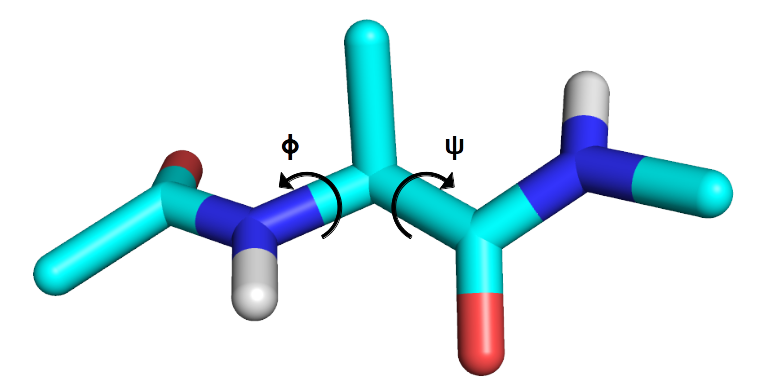
\includegraphics[scale=.3]{../07_tutorial_04/figures/aladip}
\caption{Stick representation of alanine dipeptide with the $\phi$ and $\psi$ dihedrals highlighted.}
\label{aladip}
\end{figure}
 
The preparation of the topology, coordinates, the energy minimization and the equilibration of the system follow the same procedure as described in tutorial 1.
The final equilibrated structure can be found in the directory \texttt{eq} with the name \texttt{aladip\_equilibrated.cnf}.

\subsubsection{GaMD regions definition}
The first step to perform GaMD simulations is to create a GaMD input file containing all the information of which groups of interactions to accelerate and how they need to be accelerated. 
On the directory \texttt{gamd\_setup}, you will find two files, one with the definitions to run standard GaMD, \texttt{ala.gamd}, and one showcasing the selective GaMD functionality, \texttt{selective\_ala.gamd}. Take a look to the block \texttt{GAMDATOMS} of both files.
\begin{lstlisting}
# Standard GaMD:
-----------------------------
GAMDATOMS
1
#  INATOM   FINATOM   AGROUP      
        1      3840        1
END
------------------------------
# Selective GaMD:
------------------------------
GAMDATOMS
2
#  INATOM   FINATOM   AGROUP      
        1        12       1
       13      3840       2
END
------------------------------
\end{lstlisting}
With \texttt{GAMDATOMS} you specify the number of groups of atoms to account for separately. The next line indicates the index of the first atom of the group, \texttt{INATOM}, the final atom, \texttt{FINATOM}, and an integer that will be assigned to that group, \texttt{AGROUP}, (groups of atoms with the same \texttt{AGROUP} index will be considered a single group). In the case of standard GaMD, only one set of atoms is defined. For selective GaMD, the user can define as many atom groups as desired. In the case of this tutorial, two atom groups are defined, one containing the solute (\texttt{AGROUP} = 1), and one containing the solvent (\texttt{AGROUP} = 2).
Now take a look at the second block of the \texttt{.gamd} files.
\begin{lstlisting}
# Standard GaMD:
-----------------------------
GAMDGROUPS
1
# AGROUP_1   AGROUP_2   ACCELGROUP
  1          1          1
END
------------------------------
# Selective GaMD:
------------------------------
GAMDGROUPS
1
# AGROUP_1   AGROUP_2    ACCELGROUP
  1          1           1
  1          2           1
END
------------------------------
\end{lstlisting}
This block defines the number of acceleration potentials to use, and to which interactions they should be applied.
In a similar fashion as with the previous block, \texttt{GAMDGROUPS} specifies the number of distinct acceleration potentials to use. 
The next lines assigns each group of interactions to their corresponding acceleration group were \texttt{AGROUP\_1} and \texttt{AGROUP\_2}  are the indexes of the atom groups defined in the previous block and \texttt{ACCELGROUP} is the index for the acceleration potential. 
In the case of standard GaMD, we have only one acceleration group containing the interactions of all the atoms of the system. For the selective GaMD, the interactions of the alanine didpeptide with itself (\texttt{AGROUP\_1} = 1, \texttt{AGROUP\_2} = 1) and the interactions of the alanine dipeptide with the solvent (\texttt{AGROUP\_1} = 1, \texttt{AGROUP\_2} = 2) are assigned to one acceleration group. The interactions of the solvent with itself (\texttt{AGROUP\_1} = 2, \texttt{AGROUP\_2} = 2) are not assigned to any group and thus not accelerated. The same behaviour can be obtained by using \texttt{ACCELGROUP} = 0, which is never accelerated.

\subsubsection{Acceleration parameter search}
In order to get the acceleration parameters (E and K) a search simulation needs to be performed. The search starts with a conventional MD (cMD) simulation in which the necessary statistics are recorded. After the cMD search, a starting set of E and K parameters is computed and applied to the system. After an equilibration phase, the statistics are collected again and the acceleration parameters are constantly updated. After the adaptive GaMD search, the final acceleration parameters are collected to be used for the production simulations. In this tutorial we will use 0.1 ns of cMD search followed by 0.3 ns of GaMD search. For a real case scenario the search phase must be run for longer times, at least 10 times longer than the searches described here.
Go to the directory \texttt{search}, in there you will find two directories, one for the search of the standard GaMD methodology \texttt{gamd}, and one for the selective approach \texttt{selective\_gamd}. Take a look at the \texttt{GAMD} block of the input file.
\begin{lstlisting}
GAMD
  1
# SEARCH  FORM  THRESH  NTIGAMDS
       1     1       1        1
# AGROUPS  IGROUPS
       1    1
# DIHSTD  TOTSTD
  24.79   24.79
#ED
  0
#ET
  0
#KD
  0
#KT
  0
#EQSTEPS
  0
#WINDOW
  0
END
\end{lstlisting}
The fourth line specifies the general parameters for the GaMD simulation, such as the search algorithm to use (\texttt{SEARCH}), whether the dihedral term has to be accelerated by separate (\texttt{FORM}), whether the energy threshold used is an upper or lower bound (\texttt{THRESH}), and whether the search needs to be initialized (\texttt{NTIGAMDS}). For this tutorial we will accelerate dihedral and potential term by separate (dual boosting approach) and the energy threshold will be set at the lower bound (E = $V_{max}$). 
The next line contains the number of atom groups and interaction groups or acceleration groups defined in the gamd file.
\texttt{DIHSTD} and \texttt{TOTSTD} correspond to the values of $\sigma_0$ for the dihedral term boosting and the potential term boosting respectively.  
The variables ED, ET, KD and KT are the acceleration parameters that define the boosting potential that will be applied to the system. ED and ET correspond to the list of energy thresholds for the dihedral terms and the potential energy of the system respectively, while KD and KT correspond to the list of force constants of the boosting potential applied to the dihedral term and to the potential energy term. Since this is a search run, all the parameters can be set to 0, for a production run, this parameters will need to be updated for the ones found during the search. Since each acceleration region requires its own parameters, if more than one acceleration region is defined, one must provide extra ED, ET, KD and KT parameters.
Finally, \texttt{EQSTEPS}  correspond to the number of equilibration steps to use before starting to collect statistics of the search simulation and \texttt{WINDOW} is the size of the window to use to collect the parameters, when \texttt{WINDOW} equals 0 the whole simulation is used to compute the needed statistics.

All input files are now prepared and we can generate the run file with:
\begin{lstlisting}
$ mk_script @f mkscript_gamd_search.arg
\end{lstlisting}
The job file \texttt{gamd\_search.jobs} provided to mk\_script shows the parameters that change between search runs.

For this tutorial we provide two mk\_script libraries, one to prepare the run files for a cluster using SLURM as a queueing system (\texttt{libs\/mkscript.lib}), and one for running the simulations locally, (\texttt{libs\/mkscript\_local.lib}). If the CUDA acceleration code is to be used, one simply needs to uncomment the block \texttt{INNERLOOP} from the imd files before running mk\_script.

After running the GaMD simulation, we can extract the acceleration parameters by using \texttt{ene\_ana}. The analysis files are provided in the folder \texttt{ana}.
We will use this program to read out the energy thresholds and force constants from the last energy trajectory.

You can run the program with 
\begin{lstlisting}
$ ene_ana @f ene_ana.arg
\end{lstlisting}

The file \texttt{ene\_ana.arg} contains the information of which parameters to extract from the energy trajectory. The definitions of those parameters can be found on the library file \texttt{ene\_ana.md++.lib}. This program will generate the trajectories of the selected parameters. The name of the parameters use the following syntax, "gamd\_" (to indicate that is a gamd parameter), followed by parameter to extract (in lower case), followed by the number of the acceleration region. For example, the energy threshold for the dihedrals (ED) for the first acceleration group, will be \texttt{gamd\_ed1}.

\subsubsection{GaMD production run}
Now that the search is complete we can run the production run.
Go to the directory \texttt{prod}. In a similar fashion to the \texttt{search} directory, there you will find two directories, one for the standard GaMD methodology \texttt{gamd}, and one for the selective approach \texttt{selective\_gamd}. 
The same imd used in the search runs can be used for the production ones. However, the search algorithm needs to be turned off (\texttt{SEARCH} = 0) and the acceleration parameters obtained from the search run need to be added in. 
For this tutorial, since the search run was not long enough to obtained optimal acceleration parameters, the imd files already contain all the acceleration parameters needed in them, estimated from a longer GaMD search. We will run a production simulation for a total of 1ns, although a true production run must be much longer.

The run files can be created in the same way as in the search runs by using mk\_script with its corresponding .arg file.

\subsubsection{GaMD analysis}

All the analyses for the GaMD simulations will be performed in the subfolder \texttt{ana}. 
In this section of the tutorial we will calculate the reweighted PMF for the $\phi$ and $\psi$ dihedrals of the alanine dipeptide. The same procedure can be used with any other collective variable of interest.
To extract the dihedral angle time series, first we need to run the program \textt{tser} with the correct argument files. You will find two argument files in the folder, on for each dihedral of interest, eg: \texttt{phi\_dihedral\_tser.arg}.
 \begin{lstlisting}
$ tser @f phi_dihedral_tser.arg > phi.out
\end{lstlisting}

The argument files already contain the information needed to compute the dihedrals over time accounting for periodicity, providing values from -180 to 180 degrees.
The next step is to extract the trajectory of the biasing potential used to then be able to reweight the obtained dihedral time series. This can be achieved by using the program \texttt{ene\_ana} in a similar fashion to how the acceleration parameters from the search were extracted. The values of interest are \texttt{totgamd\_dV} which contains the total boosting potential in $kJ/mol$, \texttt{totunbiased} which contains the total potential energy excluding the boosting potential and \texttt{totpot} which contains the total potential energy. The boosting potential for each acceleration region can also be extracted independently by adding \texttt{gamd\_dVi} to the ene\_ana property list  @prop with the \texttt{i} sub-index indicating the acceleration group of interest.
After obtaining the collective variables (CV) and biasing potential trajectories, the next step is to reweight and plot them. We will do this using both exponential reweighting and cumulant expansion to the second order.
In the exponential reweighting, the time series of observed values of X (in this case the dihedral angles) sampled during the biased simulation R can be reweighted to the unbiased state Y using the following equation:

\begin{equation}
  \begin{aligned}
 \langle X \rangle_Y = \frac {\langle X \exp \left[-\beta \left (V_Y - V_R \right) \right] \rangle_R} {\langle \exp \left[-\beta \left (V_Y - V_R \right) \right] \rangle_R} = \langle X \exp \left[-\beta \left (V_Y - V_R -\Delta F_{YR} \right) \right] \rangle_R
\end{aligned}
\end{equation}
where $\Delta F_{YR} = F_{Y} - F_{R}$.

The gromos toolkit offers a program called \texttt{reweight} that can be used to reweight time series of observed properties and produce a histogram of the selected number of bins. During the reweightening process special care is taken in order to avoid overflow \cite{berg2003multicanonical}. A sample input file is provided under the name of \texttt{reweight.arg}. Note that the reweight program only accepts a single time series at a time. The script \texttt{ExponentialReweighing.py} provided in the \texttt{scripts} folder can be used to reweigh the probability distribution of interest $p_{R}(\phi, \psi)$. \texttt{ExponentialReweighing.py} first discretizes the two dimensional dihedral angle matrix into a one dimensional time series. The probability distribution of this time series is then computed and reweighted using the \texttt{reweight} program. Finally, the one dimensional reweighted probability distribution is mapped back to a two dimensional probability distribution, $p_{Y}(\phi, \psi)$, and converted to energies to be able to plot them.
 \begin{lstlisting}
$ python ExponentialReweighing.py --cv1 phi.out --cv2 psi.out --vr totpot.dat --vy totunbiased.dat --xdim -180 180 10 --ydim -180 180 10
\end{lstlisting}

An alternative way of reweighting the trajectories would be to use cumulant expansion to the second order to approximate the reweighting factor. The reweighted free energy  $F_{Y}(\phi, \psi)$ will then be calculated as:
\begin{equation}
  \begin{aligned}
 F_{Y}(\phi, \psi) = F_{R}(\phi, \psi) - \sum_{k=1}^{2} \frac{\beta^{k}}{k!}C_{k} + F_{c}
\end{aligned}
\end{equation}
where $F_{c}$ is a constant, $F_{R}(\phi, \psi)$ is the free energy obtained from the unreweighted trajectory, $F_{R}(\phi, \psi) = -k_{B}T \ln{p_{R}(\phi, \psi)}$ and the first two cumulants are:
\begin{equation}
  \begin{aligned}
C_{1} = \langle \Delta V \rangle,\\
C_{2} = \langle \Delta V^2 \rangle - \langle \Delta V \rangle^2 = \sigma^{2}_{v}
\end{aligned}
\end{equation}
This can be achieved by using the pyreweight script that is provided in the \textttt{scripts} directory or that can be downloaded from its original repository \cite{miao2014improved}.

The version provided in the \textttt{scripts} folder contains a small modification to provide the results in kJ/mol to ease the comparison to the results provided by GROMOS. The script takes as input a file with the CVs in columns and another file with the biasing potential with three columns, biasing in kJ/mol, time, and biasing in kcal/mol. An example of how to run the script can be found on the \textttt{scripts} folder on the file \textttt{pyreweight\_command.txt}.

Because the performed trajectories are too short to obtain converged PMFs, the dihedral and energy trajectories of a 100 ns run are provided in the subfolder \texttt{data}. The same analysis can be performed on the files provided there, producing the 2D-PMFs in figure \ref{aladip_pmf}:

\begin{figure}[H]
\centering
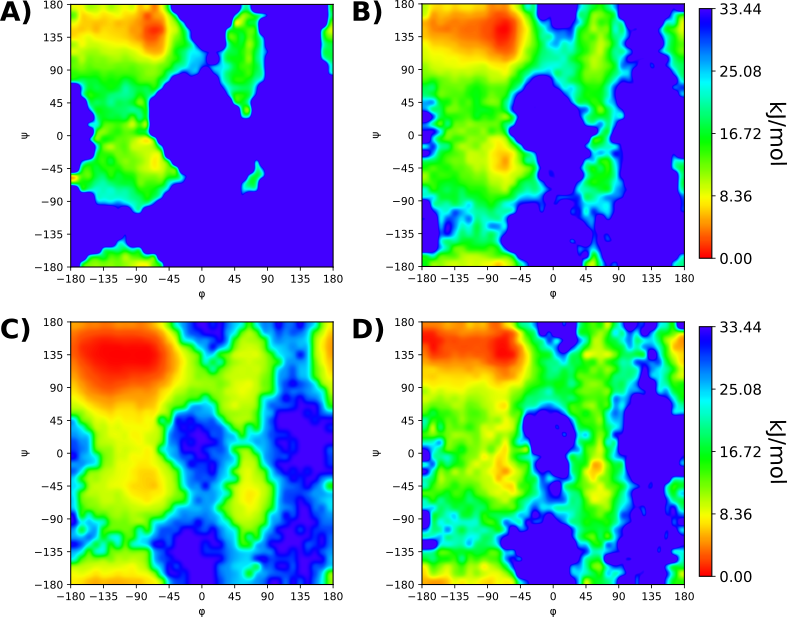
\includegraphics[scale=.43]{../07_tutorial_04/figures/pmf_tutorial}
\caption{Potential of Mean Force (PMF) profiles over the $\phi$ and $\psi$ angles of the alanine dipeptide. A) Simulation using the standard GaMD approach reweighted with cumulant expansion to the second order. B) Simulation using the standard GaMD approach reweighted with exponential reweighing. C) Simulation using the selective GaMD approach reweighted with cumulant expansion to the second order. D) Simulation using the selective GaMD approach reweighted with exponential reweighing. }
\label{aladip_pmf}
\end{figure}



